% \usepackage[margin=2cm]{geometry}


% \begin{tikzpicture}
\begin{tikzpicture}
\filldraw
(0,0) circle (2pt) node[align=center,below] {$ 0 $} --
(3.81,0) circle (2pt) node[align=center,below] {$ \sigma \approx 0.381 $} -- 
(6.18,0) circle (2pt) node[align=center,below] {$ \tau  \approx 0.618 $} --
(10,0) circle (2pt) node[align=center,below] {$ 1 $};
% \draw[-][very thick] (0,0) -- (1,0);
% \draw [thick] (0,-.1) node[below]{0} -- (0,0.1);
% \draw [thick] (0.381,-.1) node[below]{$ \sigma \approx 0.381 $} -- (0.381,0.1);
% \draw [thick] (0.381,-.1) node[below]{$ \tau \approx 0.618 $} -- (0.618,0.1);
% \draw [thick] (1,-.1) node[below]{1} -- (1,0.1);
\end{tikzpicture}

% \begin{tikzpicture}
% \draw(0,0)--(10,0);
% \foreach \x/\xtext in {1/$ \ sigma $,2/$ \tau1$,4/$ 1$,6/$0$,8/$m$,10/$m+n-1$}
%     \draw(\x,5pt)--(\x,-5pt) node[below] {\xtext};
% \draw[decorate, decoration={brace}, yshift=2ex]  (0,0) -- node[above=0.4ex] {$0$'s}  (2,0);
% \draw[decorate, decoration={brace, mirror}, yshift=2ex]  (10,0) -- node[above=0.4ex] {$l$'s and $0$'s with $l$'s separated by at least two $0$'s}  (4,0);
% \end{tikzpicture}

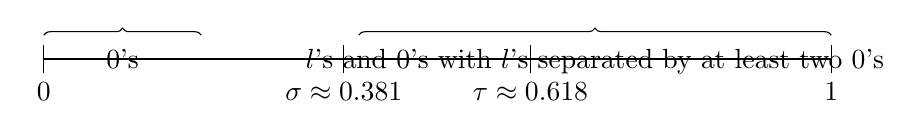
\begin{tikzpicture}
\draw(0,0)--(10,0);
\draw(0,5pt)--(0,-5pt) node[below] {$ 0 $};
\draw(3.81,5pt)--(3.81,-5pt) node[below, align=left] {$ \sigma \approx 0.381 $};
\draw(6.18,5pt)--(6.18,-5pt) node[below, align=left] {$ \tau \approx 0.618 $};
\draw(10,5pt)--(10,-5pt) node[below] {$ 1 $};
\draw[decorate, decoration={brace}, yshift=2ex]  (0,0) -- node[below=0.4ex] {$0$'s}  (2,0);
\draw[decorate, decoration={brace, mirror}, yshift=2ex]  (10,0) -- node[below=0.4ex] {$l$'s and $0$'s with $l$'s separated by at least two $0$'s}  (4,0);
\end{tikzpicture}


\begin{tikzpicture}
\begin{axis}[axis lines=left, xlabel=$x$, ylabel={$f(x)$}, xmin=-5, xmax=5, ymin=0, ymax=5]
\addplot[domain=-10:10,samples=100,color=red]{(x - 2)^2 + 1};
\addlegendentry{$ {(x - 2)}^2 + 1 $}
\addplot[domain=-10:10, samples=100, color=blue]{x^2};
\addlegendentry{$ x^2 $}
\end{axis}
\end{tikzpicture}

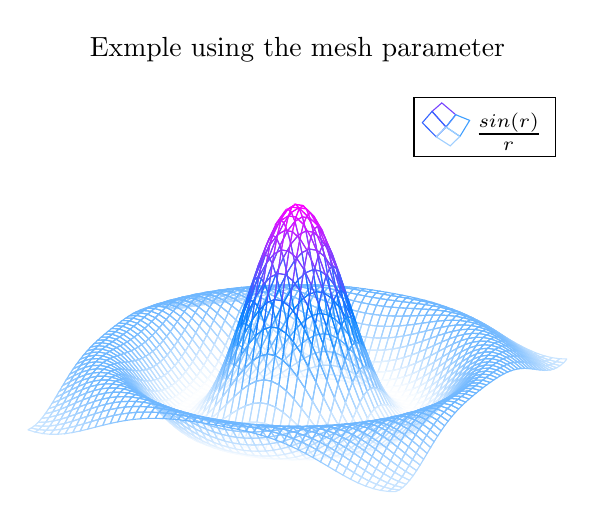
\begin{tikzpicture}
\begin{axis}[
    title=Exmple using the mesh parameter,
    hide axis,
    colormap/cool,
]
\addplot3[
    mesh,
    samples=50,
    domain=-8:8,
]
{sin(deg(sqrt(x^2+y^2)))/sqrt(x^2+y^2)};
\addlegendentry{$\frac{sin(r)}{r}$}
\end{axis}
\end{tikzpicture}

% simple x^2
\begin{tikzpicture}
\begin{axis}[axis lines=left, xlabel=$x$, ylabel={$f(x)$}, xmin=-5, xmax=5, ymin=0, ymax=5]
\addplot[domain=-10:10,samples=100,color=red]{(x - 2)^2 + 1};
\addlegendentry{$ {(x - 2)}^2 + 1 $}
\addplot[domain=-10:10, samples=100, color=blue]{x^2};
\addlegendentry{$ x^2 $}
\end{axis}
\end{tikzpicture}


% sort of works
\begin{figure}[H]
\centering
\begin{tikzpicture}

\coordinate[label={150:$A$}] (A) at (135:4);
\coordinate[label={270:$C$}] (C) at (0:0);
\coordinate[label={30:$B$}] (B) at (45:5);
\draw (C) -- (A)node[midway,below left]{$b$} -- (B)  -- cycle node[midway,below right]{$a$};
\draw (C) -- ($(A)!(C)!(B)$) coordinate (P) node[midway,right]{$h$};
\draw[decorate,decoration={brace,raise=12pt,amplitude=5pt}] (A) -- (B);
\path (B) -- (P) node[midway,above]{$x$} -- (A) node[midway,above]{$y$} ($($(A)!0.5!(B)$)!0.8cm!90:(B)$) node{$C$};
\filldraw[fill=white] (C) -- ($(C)!2mm!(A)$) coordinate (U) -- ($(U)!2mm!90:(C)$) --($(C)!2mm!(B)$) --cycle;
\draw ($(P)!2mm!(C)$) coordinate (V) -- ($(V)!2mm!90:(C)$) --($(P)!2mm!(B)$);

\end{tikzpicture}
\caption{Pythagoras}\label{fig:pythagoras} 
\end{figure}
\bigskip


